\documentclass[12pt]{article}
\usepackage[a4paper, margin=2.5cm]{geometry}
\usepackage{lmodern}
\usepackage{hyperref}
\usepackage{longtable}
\usepackage{titlesec}
\usepackage{graphicx}
\usepackage{enumitem}
\usepackage{float}
\usepackage{booktabs} 
\titleformat{\section}{\normalfont\large\bfseries}{\thesection}{1em}{}
\newcommand{\sectionbreak}{\clearpage}
%nina note: strg,alt,b to build

\title{Refined Project Plan\\\large infrared.city-1: Tree detection}
\author{
Moritz Hörmansdorfer (h12417021) \\
Sara Klasová (h12122714) \\
Dominik Oberhumer (h01025454) \\
Nina Salnikow (h12109432) \\
}
\date{\today}

\begin{document}

\maketitle

\section{Project Description}

This chapter outlines the motivation, methods used, data sources and the scope of this project.

\subsection{Motivation and Project Overview}

As urban areas are expanding and global temperatures rise due to climate change, being able to understand how trees can help cool cities has become increasingly important \cite{eu2023tree}. Furthermore, trees reduce the risk of flooding in cities and promote health and wellbeing \cite{woodlandtrust2023}. Our project aims at taking the first step in the direction of better tree coverage in urban areas by creating a model which is able to predict tree locations using satellite imagery of densely populated areas. \\
\\
There is a recently very fast growing body of reasearch on urban tree detection using deep learning models. One of the most recent papers is by Gong et al. \cite{gong2024treedetector}, they use satellite data not only to detect trees but also to estimate their size and density. For that they use a slightly different model then the U-Net model used in this paper.

\subsection{Data Sources}

For our project we use publicly available Sentinel-2 satellite images with 10-meter spatial resolution and four color channels, namely red, green, blue and near infrared. The images are retrieved via the API of the Copernicus Programme and are provided by the European Space Agency \cite{copernicus2025}. As seasonality has a great impact on the appearance of trees, imagery of different seasons will be used to train the model. \\
\\
Additionally, we will use the publicly available data set on every tree in the city of Vienna “Baumkataster” to train and test our model on exact tree locations \cite{baumkataster2025}.

\subsection{Model}

Former papers suggest that for image segmentation with satellite data the U-Net deep learning model is the most accurate for detecting objects, for example street detection \cite{pesek2024convolution} as well as crop field detection \cite{garnot2021panoptic}. Furthermore, last year's project also tried implementing a U-Net architecture but failed to yield promising results and this paper tries to build on that, especially because the data coaches also deem it a well-fitting model. This architecture will therefore also be used in this paper to predict tree locations. \\
\\
The U-Net model is a special type of Convolutional Neural Network and consists of a contracting path and an expanding path. In the contracting path convolution and pooling layers are used to extract features from the original imagery, which in this project will consist of four pictures for each season and four color channels each as described above. The expanding path consists of the same structure of convolution and pooling layers but used in the other direction to up-sample the before contracted imagery \cite{aramendia2024}. As suggested in similar work this project will use skip connections between the expanding and contracting path as well as a temporal attention algorithm to prioritize more meaningful images \cite{garnot2021panoptic}. The Binary Cross-Entropy loss between the predicted locations will be used and the actual locations from the “Baumkataster” will be split into a train and test set.

\subsection{Project Scope and Possible Limitations}

The model in this paper is trained only on satellite images of urban areas and therefore also only supposed to be used for tree detection within city environments. Also, the model focuses on tree detection in the temperate climate zone as this is the vegetation it is trained to observe. Further analysis on the impact of trees on, for example, heat regulation in cities and flooding prevention are out of the scope of this project and could be the topic of future research. \\
\\
As this paper uses Sentinel-2 satellite images with 10-meter spatial resolution this could lead to issues as the images might not have a high enough resolution to detect trees reliably. Future work could therefore also focus on improving the image quality with better available satellite data.

\section{BEAM}

Figure~\ref{fig:beam} presents the BEAM representation of the proposed tree detection system, illustrating the data sources, training and inference processes, model architecture, evaluation pipeline, and associated risks.

\begin{figure}[H] 
    \centering
    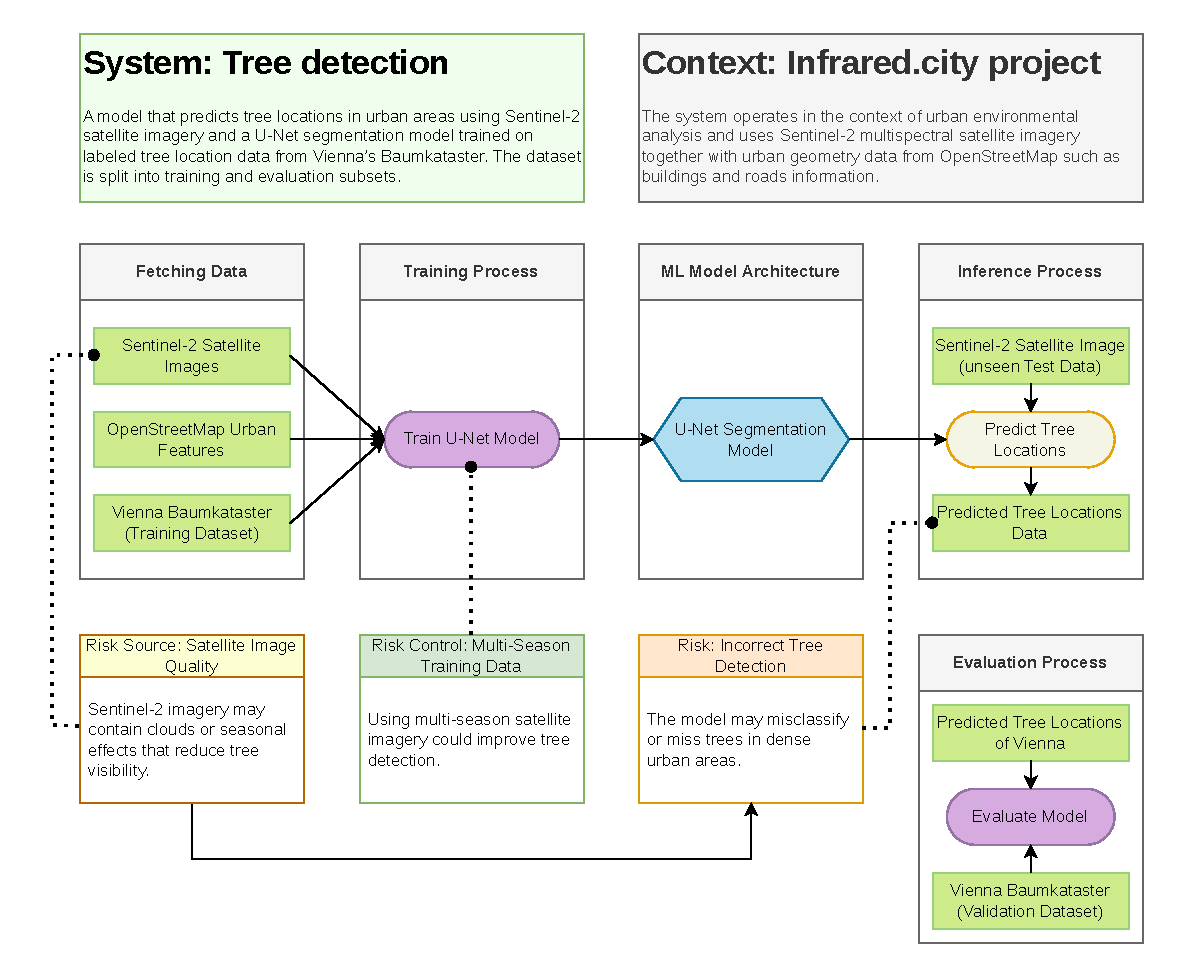
\includegraphics[width=\textwidth]{beam_treeDetection_infraredCity.pdf}
    \caption{BEAM model of the proposed tree detection system.}
    \label{fig:beam}
\end{figure}


\section{Timeplan}

This chapter descripes our planned timeline

\subsection{Milestones}

The project will be conducted between March and June and is structured into several phases corresponding to the course milestones and deliverables.

\subsubsection[Phase 1: Project Setup \& Planning]{Phase 1: Project Setup \& Planning \\ \normalsize March 9 – March 19}
This initial phase focuses on defining the project scope, exploring available data sources, and establishing a solid project plan.

\begin{description}[style=multiline, leftmargin=3cm, font=\normalfont\textbf]
    \item[Tasks:] 
    \begin{itemize}[nosep, leftmargin=*]
        \item Kick-off session and first meeting with data coaches (March 9)
        \item Define project objective and research question
        \item Explore available datasets (Sentinel-2, OpenStreetMap, etc.)
        \item Decide on modelling approach
        \item Assign team roles
        \item Draft project plan
    \end{itemize}
    \item[Deliverable:] Project Plan -- March 19
\end{description}

\subsubsection[Phase 2: Methodology Development]{Phase 2: Methodology Development \\ \normalsize March 20 – March 29}
During this phase, the primary goal is to acquire the necessary data and establish the foundational methodology for feature extraction.

\begin{description}[style=multiline, leftmargin=3cm, font=\normalfont\textbf]
    \item[Tasks:] 
    \begin{itemize}[nosep, leftmargin=*]
        \item Data collection and preprocessing
        \item Feature extraction (spectral indices, vegetation signals)
        \item Define modelling pipeline
        \item Improve project plan based on feedback
    \end{itemize}
    \item[Deliverable:] Refined Project Plan -- March 29
\end{description}

\subsubsection[Phase 3: Data Processing \& Initial Modelling]{Phase 3: Data Processing \& Initial Modelling \\ \normalsize March 30 – April 21}
This period is dedicated to executing the data processing pipeline and training the first iteration of machine learning models.

\begin{description}[style=multiline, leftmargin=3cm, font=\normalfont\textbf]
    \item[Tasks:] 
    \begin{itemize}[nosep, leftmargin=*]
        \item Implement data processing pipeline
        \item Train initial machine learning models
        \item Evaluate early results
        \item Prepare intermediate analysis
        \item Create presentation slides
    \end{itemize}
    \item[Deliverable:] Intermediate Report and Slides -- April 21
\end{description}

\subsubsection[Phase 4: Model Improvement \& Validation]{Phase 4: Model Improvement \& Validation \\ \normalsize April 22 – June 6}
Focus now shifts towards optimizing model performance through rigorous validation, error analysis, and peer feedback.

\begin{description}[style=multiline, leftmargin=3cm, font=\normalfont\textbf]
    \item[Tasks:] 
    \begin{itemize}[nosep, leftmargin=*]
        \item Intermediate consultations (April 22–24)
        \item Improve model performance
        \item Perform validation and error analysis
        \item Conduct sparring group meetings
        \item Prepare final report draft
    \end{itemize}
    \item[Deliverable:] Draft Final Report \& Slides -- June 7
\end{description}

\subsubsection[Phase 5: Finalization \& Presentation]{Phase 5: Finalization \& Presentation \\ \normalsize\ June 8 – June 28}
The final phase encompasses the conclusive evaluation of the models and the preparation of the final deliverables and class presentations.

\begin{description}[style=multiline, leftmargin=3cm, font=\normalfont\textbf]
    \item[Tasks:] 
    \begin{itemize}[nosep, leftmargin=*]
        \item Final model evaluation
        \item Prepare final presentation
        \item Final presentation in class (June 18–19)
        \item Final report writing and revisions
        \item Submit sparring group minutes
    \end{itemize}
    \item[Deliverables:] 
    \begin{itemize}[nosep, leftmargin=*]
        \item Final Report -- June 28
        \item Sparring Group Minutes -- June 28
    \end{itemize}
\end{description}

\subsection{Tasks}

Following in Table~\ref{tab:project_timeline} we have our first export of our current ticket. The export was done on 28. March 2026. 
This tickets are our current state of plan who will do what and when. The table is structured by the major milestone phases.
In some cases we dont have one specific assignee for tasks. In this cases we mentioned right now multiple persons for a specific task, and we have to descide at time how to split up this task on the given list of persons. For example the writting of the report can be structured as subtask by topic and everybody writtes different chapters. But right now we are not sure about the existing topics. So we desicded that in our current state it is enough to use multiple assignees.

\begin{longtable}{@{} p{5.5cm} p{5cm} l l l @{}}
\caption{Project Timeline and Task Assignments} \label{tab:project_timeline} \\
\toprule
\textbf{Task} & \textbf{Assignee(s)} & \textbf{Status} & \textbf{Start} & \textbf{End} \\
\midrule
\endfirsthead

\multicolumn{5}{c}%
{{\bfseries Table \thetable\ continued from previous page}} \\
\toprule
\textbf{Task} & \textbf{Assignee(s)} & \textbf{Status} & \textbf{Start} & \textbf{End} \\
\midrule
\endhead

\midrule
\multicolumn{5}{r}{{Continued on next page}} \\
\endfoot

\bottomrule
\endlastfoot

% --- Project Plan ---
\multicolumn{5}{@{}l}{\textbf{Project Plan}} \\ \midrule
Setup Git Repository & Dominik Oberhumer & Done & 10.03.2026 & 13.03.2026 \\
Kickoff Session & Moritz Hörmansdorfer, Dominik Oberhumer, Nina Salnikow, Sara Klasová & Done & 13.03.2026 & 13.03.2026 \\
Initialize Latex Template & Dominik Oberhumer & Done & 13.03.2026 & 14.03.2026 \\
Explore Datasets & Nina Salnikow & Done & 13.03.2026 & 15.03.2026 \\
Explore Modelling Approaches & Moritz Hörmansdorfer, Sara Klasová & Done & 13.03.2026 & 16.03.2026 \\
Write Project Plan Project Description & Moritz Hörmansdorfer & Done & 14.03.2026 & 18.03.2026 \\
Write Project Plan BEAM & Nina Salnikow & Done & 14.03.2026 & 18.03.2026 \\
Write Project Plan Timeplan & Sara Klasová & Done & 14.03.2026 & 18.03.2026 \\
Write Project Plan Communication & Dominik Oberhumer & Done & 14.03.2026 & 18.03.2026 \\
Write Project Plan Team Roles & Dominik Oberhumer & Done & 14.03.2026 & 18.03.2026 \\
Write Project Plan Literature & Sara Klasová & Done & 14.03.2026 & 18.03.2026 \\
\addlinespace

% --- Refined Project Plan ---
\multicolumn{5}{@{}l}{\textbf{Refined Project Plan}} \\ \midrule
Refine Project Plan Project Description & Moritz Hörmansdorfer & In Prog. & 19.03.2026 & 29.03.2026 \\
Refine Project Plan BEAM & Nina Salnikow & In Prog. & 19.03.2026 & 29.03.2026 \\
Refine Project Plan Timeplan & Dominik Oberhumer & In Prog. & 19.03.2026 & 29.03.2026 \\
Refine Project Plan Communication & Dominik Oberhumer & In Prog. & 19.03.2026 & 29.03.2026 \\
Refine Project Plan Team Roles & Dominik Oberhumer & In Prog. & 19.03.2026 & 29.03.2026 \\
Refine Project Plan Literature & Sara Klasová & In Prog. & 19.03.2026 & 29.03.2026 \\
Collect Data Baumkataster & Nina Salnikow & Done & 19.03.2026 & 28.03.2026 \\
Collect Data from Copernicus & Nina Salnikow & Todo & 19.03.2026 & 28.03.2026 \\
Collect Data additional Data sources? & Nina Salnikow & In Prog. & 19.03.2026 & 28.03.2026 \\
Define modelling pipeline & Moritz Hörmansdorfer, Nina Salnikow, Sara Klasová & Todo & 19.03.2026 & 02.04.2026 \\
Prepare Data Baumkataster (Features) & Nina Salnikow & Todo & 29.03.2026 & 02.04.2026 \\
Prepare Data Copernicus (Features) & Nina Salnikow & Todo & 29.03.2026 & 02.04.2026 \\
Prepare Data additional Data Sets? & Nina Salnikow & Todo & 29.03.2026 & 02.04.2026 \\
\addlinespace

% --- Intermediate Report ---
\multicolumn{5}{@{}l}{\textbf{Intermediate Report}} \\ \midrule
Schedule minutes with sparing team & Dominik Oberhumer & Todo & 30.03.2026 & 16.04.2026 \\
Define structure of report & Dominik Oberhumer & Todo & 30.03.2026 & 04.04.2026 \\
EDA & Sara Klasová & Todo & 03.04.2026 & 09.04.2026 \\
Implement data processing pipeline & Moritz Hörmansdorfer, Nina Salnikow, Sara Klasová & Todo & 03.04.2026 & 09.04.2026 \\
Create latex template for report & Dominik Oberhumer & Todo & 05.04.2026 & 08.04.2026 \\
Write intermediate project report & Moritz Hörmansdorfer, Dominik Oberhumer, Nina Salnikow, Sara Klasová & Todo & 09.04.2026 & 21.04.2026 \\
Prepare Slides for presentation & Moritz Hörmansdorfer, Dominik Oberhumer, Nina Salnikow, Sara Klasová & Todo & 09.04.2026 & 21.04.2026 \\
Train initial machine learning models & Moritz Hörmansdorfer & Todo & 10.04.2026 & 17.04.2026 \\
Evaluate early results & Moritz Hörmansdorfer & Todo & 10.04.2026 & 17.04.2026 \\
Prepare intermediate analysis & Moritz Hörmansdorfer, Dominik Oberhumer, Nina Salnikow, Sara Klasová & Todo & 12.04.2026 & 17.04.2026 \\
\addlinespace

% --- Draft Final Report & Slides ---
\multicolumn{5}{@{}l}{\textbf{Draft Final Report \& Slides}} \\ \midrule
Prepare latex for Draft Final Report & Dominik Oberhumer & Todo & 21.04.2026 & 25.04.2026 \\
Improve model performance & Moritz Hörmansdorfer, Sara Klasová & Todo & 22.04.2026 & 21.05.2026 \\
Define Resulted Database Structure & Moritz Hörmansdorfer, Dominik Oberhumer, Nina Salnikow, Sara Klasová & Todo & 22.04.2026 & 03.05.2026 \\
Sparring group meetings & Moritz Hörmansdorfer, Dominik Oberhumer, Nina Salnikow, Sara Klasová & Todo & 22.04.2026 & 05.06.2026 \\
Write Draft Final Report & Moritz Hörmansdorfer, Dominik Oberhumer, Nina Salnikow, Sara Klasová & Todo & 26.04.2026 & 07.06.2026 \\
Perform validation and error anylsis & Sara Klasová & Todo & 28.04.2026 & 31.05.2026 \\
Invite data coaches to presentation & Dominik Oberhumer & Todo & 03.05.2026 & 09.05.2026 \\
Implement Resulted Database & Moritz Hörmansdorfer, Sara Klasová & Todo & 04.05.2026 & 31.05.2026 \\
Prepare Slides for final presentation & Moritz Hörmansdorfer, Dominik Oberhumer, Nina Salnikow, Sara Klasová & Todo & 10.05.2026 & 07.06.2026 \\
\addlinespace

% --- Final Report ---
\multicolumn{5}{@{}l}{\textbf{Final Report}} \\ \midrule
Prepare latex template for final report & Dominik Oberhumer & Todo & 06.06.2026 & 09.06.2026 \\
Prepare official sparring group minutes & Nina Salnikow & Todo & 07.06.2026 & 28.06.2026 \\
Final model evaluation & Moritz Hörmansdorfer, Dominik Oberhumer, Nina Salnikow, Sara Klasová & Todo & 08.06.2026 & 21.06.2026 \\
Write final reports & Moritz Hörmansdorfer, Dominik Oberhumer, Nina Salnikow, Sara Klasová & Todo & 09.06.2026 & 28.06.2026 \\

\end{longtable}

\subsection{GANTT}

In Figure \ref{fig:gantt_chart} we have a GANTT chart showing the structure of the tasks.

\begin{figure}[htbp]
    \centering
    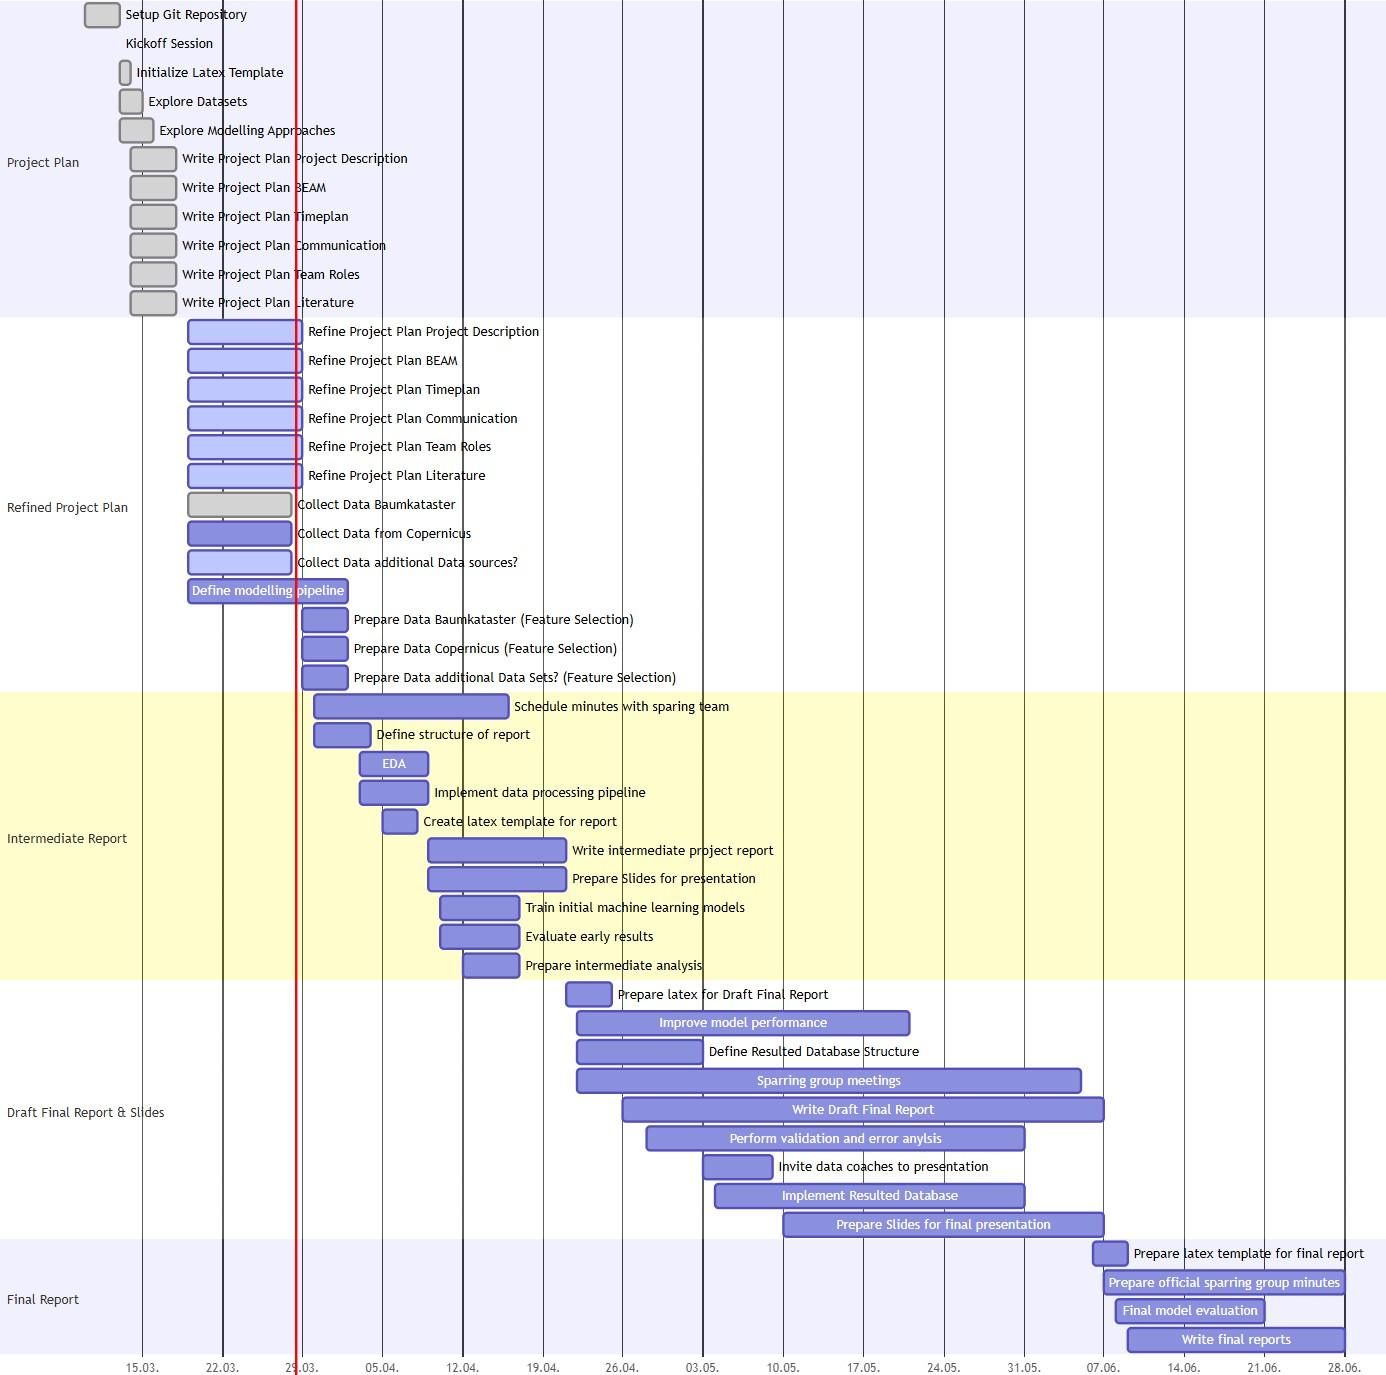
\includegraphics[width=\textwidth]{GANTT.jpg} 
    \caption{GANTT Diagramm}
    \label{fig:gantt_chart}
\end{figure}

\section{Communication outline}

This section describes the communication styles we are committed to use over the project.

\subsection{Written communication}

We will use two Teams in Microsoft Teams for our basic communication.

\begin{enumerate}
    \item \textbf{DsLab26S\_infrared.city\_1}: This Team contains two channels for two different approaches. The \textbf{General} Channel is used as communication level with Kavita Surana (our connection to the Lecture and the WU). The other channel (\textbf{team intern}) is only accessible by the team itself and is our main chat for communication over the project.
    \item \textbf{DsLab\_infrared.city\_1-coaches}: This Team is the basic for communication with the data coaches from infrared-city. We were asked to separate this from the main communication source, but still keep a Microsoft Teams Team for this. So we created a different Team.
\end{enumerate}

\subsection{Regular Meetings and Communication}

Our meetings will be held via Microsoft Teams in most cases. It is possible that we are able to meet in person for one or another defined meeting. But regularly we plan to keep the communication remote or at least hybrid. We organized already two regular weekly meetings for basic communication.

\begin{enumerate}
    \item \textbf{Regular Team Meeting}: On Thursdays 19:00 we will meet as a team remotely and talk about how to continue the work over the next week.
    \item \textbf{Irregular Meetings with Kavita Surana}: In cases we need feedback for something from the WU site we schedule a meeting with her. At least we will schedule a meeting before the major deliverables. To easily schedule the meeting we got a booking site for her time.
    \item \textbf{Communication with Data Coaches from infrared.city}: No regular meeting is scheduled with the data coaches. Instead we write weekly reports in the shared Teams channel. In most cases this weekly report will be send after our weekly regular team meeting by Dominik.
\end{enumerate}

\subsection{Documentation of Meetings}

Because of the many meetings it is possible that one or another person is not able to participate every time. To still be able to communicate with absent people we want to write meeting notes and documentation of the meeting output after every meeting. This documenation is mainly for us to be able to better remember previous decisions. The protocolls are commited to our GIT Repository, like every other written result as simple text documents containing the date and time, attended people, discussed topics and the follup up decisions.  

\subsection{File and Code Repository}

Every written result (documentation and project related) will be added to an already created GitHub repository. The repository is accessible by the team. See \url{https://github.com/nikmaster/wu_dslab_infrared-city}.

\subsection{Ticket and Issue Tracking}

We have a Project in GitHub to track our progress on issue and ticket level. This allows us to specify who is doing what and when. And also creates an easy graphical overview

\section{Team Roles}

The main project team consists of 4 persons which are responsible for different focus points. But still commit to the project and in case one person gets stuck, the focus has to be to work together and find a way to tackle the issue.

\begin{table}[htbp]
\centering
\begin{tabular}{@{}llp{6cm}@{}}
\toprule
\textbf{Person} & \textbf{Role} & \textbf{Tasks} \\
\midrule
\textbf{Dominik Oberhumer} & Organisation of Team & Preparation of Tools, Reminding of Deliverables and Timeplan \\
\textbf{Moritz Hörmansdorfer} & Data Scientist & Machine Learning Training of Model \\
\textbf{Nina Salnikow} & Data Engineer & Fetching and Preparation of Data  \\
\textbf{Sara Klasová} & Data Scientist & EDA (Exploratory Data Analysis)  \\
\bottomrule
\end{tabular}
\end{table}

Besides these persons, we also have additional support from people which are related to the project:

\begin{enumerate}
    \item \textbf{Kavita Surana}: is our supervisor from WU. She will help us regarding infrastructure and gives the needed points for grading at the university.
    \item \textbf{Oana Taut} and \textbf{Vasiliki Fragkia} are our data coaches from infrared.city. They will support us with different approaches and sources how we can use the data to achieve our goal.
\end{enumerate}


\section{Literature}

Following additional papers are planned to be used as sources:

1. A review of individual tree crown detection and delineation from optical remote sensing images \cite{zheng2023reviewindividualtreecrown}

2. Integrating Traditional and Deep Learning Methods to Detect Tree Crowns in Satellite Images \cite{durgut2025integrating}

3. A Sentinel-2 machine learning dataset for tree species classification in Germany  \cite{freudenberg2025sentinel2}

4. Object-based classification of urban plant species from very high-resolution satellite imagery \cite{sicard2023object}

5. Improving Urban Tree Species Classification with High Resolution Satellite Imagery and Machine Learning \cite{wenger2024improving}


\bibliographystyle{ieeetr} 
\bibliography{literature}

\end{document}